\documentclass[useAMS, usenatbib]{mnras}
\pdfsuppresswarningpagegroup=1
%
\usepackage[spanish,es-minimal,english]{babel}
\usepackage[utf8]{inputenc}
\usepackage{graphicx}

\usepackage{xcolor}
\usepackage{hyperref}
\usepackage{siunitx}
\usepackage{newtxtext}
\usepackage[stix2,smallerops]{newtxmath}
\usepackage{booktabs}
\hypersetup{colorlinks=True, linkcolor=blue!50!black, citecolor=black,
  urlcolor=blue!50!black}
\usepackage{etoolbox}
\robustify\bfseries
\robustify\itshape

\usepackage[shortlabels]{enumitem}

\bibliographystyle{mnras}

\sisetup{
  % explicit "+" is useful for velocities
  retain-explicit-plus = true,
  % prefer 10^6 over 1 x 10^6
  retain-unity-mantissa = false,
  % Use x +/- e instead of x(e)  
  separate-uncertainty = true,
  % Make sure to pick up bold font when used in section heading for instance
  detect-weight = true,
}

%% 
%% Will macros
%%
% A better \ion command that works in more circumstances
\newcommand\ION[2]{#1\,\scalebox{0.9}[0.8]{\uppercase{#2}}}
\newcounter{ionstage}
\renewcommand{\ion}[2]{\setcounter{ionstage}{#2}% 
  \ensuremath{\mathrm{#1\,\scriptstyle\Roman{ionstage}}}}
\newcommand\hii{\ion{H}{2}}
\newcommand\nii{[\ion{N}{2}]}
\newcommand\oiii{[\ion{O}{3}]}
\newcommand\oii{[\ion{O}{2}]}
\newcommand\Wav[1]{\ensuremath{\lambda #1}}

\title[HH 529 II and III in the Orion Nebula]{
  Photoionized Herbig-Haro objects in the Orion Nebula I: HH 529 II and III
}

\author[J. E. M\'endez-Delgado et al.]
{J. E. M\'endez-Delgado$^{1,2}$ \thanks{E-mail: jemd@iac.es},
  C. Esteban$^{1,2}$, J. Garc{\'{\i}}a-Rojas$^{1,2}$, W. J. Henney$^{3}$  
  \newauthor 
  and K. Z. Arellano-C\'ordova$^{1}$ and collaborators\\
\\
% List of institutions
$^{1}$Instituto de Astrof\'isica de Canarias (IAC), E-38205 La Laguna, Spain\\
$^{2}$Departamento de Astrof\'isica, Universidad de La Laguna, E-38206 La Laguna, Spain\\
$^{3}$Instituto de Radioastronom\'ia y Astrof\'isica, Universidad Nacional Aut\'onoma de M\'exico, Apartado Postal 3-72, 58090 Morelia, Michoac\'an, M\'exico}


\begin{document}

\begin{table}
  % Fake the labels for some Tables
  \setcounter{table}{3}\caption{}\label{tab:pc}
  \setcounter{table}{12}\caption{}\label{tab:total_abundances_rls}
\end{table}

\section{Shock emission versus shell emission}
\label{sec:shoc-v-shell}

\begin{figure}
  \centering
  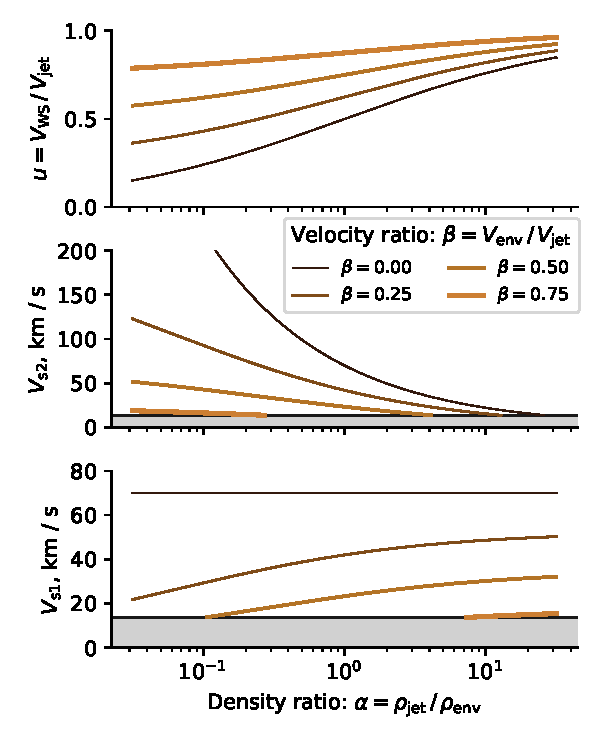
\includegraphics[width=\linewidth]{shock-velocities}
  \caption{Inner and outer shock velocities in a working surface}
  \label{fig:shock-velocities}
\end{figure}

\newcommand\Mach{\ensuremath{\mathcal{M}}}
\newcommand\shock{\ensuremath{_{\mathrm{sh}}}}
\newcommand\sound{\ensuremath{c_{\mathrm{s}}}}
Since the material in the HH outflows is moving highly supersonically
with respect to the ionized sound speed in the nebula
it will give rise to shocks where the flow and nebula interact
\citep{Hartigan:1987a}.
Further internal shocks may form inside the outflow
if its velocity varies with time \citep{Raga:1990a}.
It is important to investigate the degree to which direct excitation by the shocks
might be affecting our emission line analysis.

A hydrodynamic shock is characterized by its Mach number \(\Mach = V\shock / \sound\),
where \(V\shock\) is the shock velocity and \(\sound\) is the pre-shock adiabatic sound speed.
On passing through the shock, the gas is heated 
\citep{ZelDovich:1969a} to a temperature \(T_1\),
which is higher than the equilibrium photoionized temperature, \(T_0\):
\begin{equation}
  \label{eq:T1-T0}
  \frac{T_1}{T_0} = \frac{1}{16} \bigl( 5 \Mach^2 - 1 \bigr)
  \bigl( 1 + 3\Mach^{-2} \bigr),
\end{equation}
while at the same time it is compressed by a factor
\begin{equation}
  \label{eq:rho1-rho0}
  \frac{\rho_1}{\rho_0} = \frac{4 \Mach^2}{\Mach^2 + 3} .
\end{equation}
In both cases, a ratio of specific heats \(\gamma = 5/3\) is assumed,
as is appropriate for ionized and atomic gas. 
The post-shock gas then cools in a radiative relaxation layer
until it returns to the equilibrium temperature \(T_2 \approx T_0\),
reaching a final density compression factor of 
\begin{equation}
  \label{eq:rho2-rho0}
  \frac{\rho_2}{\rho_0} = \frac53 \Mach^2 .
\end{equation}

The adiabatic sound speed in the equilibrium ionized gas is given by
\(\sound = (\gamma k T / \mu m_{\mathrm{H}})^{1/2}\),
where \(k\) is the Boltzmann constant, \(T\) is the temperature,
\(m_{\mathrm{H}}\) is the hydrogen mass
and \(\mu\) is the mean atomic mass per particle.
Assuming that all He is singly ionized with
\(y = \mathrm{He/H} = 0.087\) (Table~\ref{tab:total_abundances_rls}) yields
\(\bar{m} \approx (1 + 4 y) / (2 + 2 y) \approx 0.62\),
which combined with \(T = \SI{8480}{K}\) (Table~\ref{tab:pc})
implies an adiabatic sound speed of \(\approx\SI{13.7}{km.s^{-1}}\). 

Clumpy jets \citep{Yirak:2009a, Yirak:2012a}.  Double working surfaces \citep{Raga:2017b}.   

Magnetic field \citep{Hansen:2017a, Pudritz:2019a}

\bibliography{will-529-shock-refs}

\end{document}

%%% Local Variables:
%%% mode: latex
%%% TeX-master: t
%%% End:
